\documentclass[11pt]{article}
\usepackage[utf8]{inputenc}
\usepackage[T1]{fontenc}
\usepackage{amsmath}
\usepackage{amssymb} % Needed for \eth
\usepackage{graphicx}
\usepackage{geometry}
\usepackage{tikz}
\usepackage{pgfplots} % For plots
\usepackage{ulem}     % For underline, using normalem to avoid messing with \emph
\usepackage{tcolorbox} % For boxing equations
\usepackage{braket}    % For QM state notation if needed
\usetikzlibrary{calc}
\geometry{a4paper, margin=1in}
\usetikzlibrary{positioning, arrows.meta, shapes.geometric} % For TikZ diagrams
\pgfplotsset{compat=1.18} % Use a recent PGFPlots version

% Custom commands (optional)
\newcommand{\avg}[1]{\overline{#1}}
\newcommand{\prob}[1]{P(#1)}
\newcommand{\ProbDens}[1]{\mathcal{P}(#1)} % Using script P for density
\newcommand{\vect}[1]{\vec{#1}}
\newcommand{\dd}[1]{\mathrm{d}#1} % Differential d
\newcommand{\pderiv}[2]{\frac{\partial #1}{\partial #2}}
\newcommand{\deriv}[2]{\frac{\mathrm{d} #1}{\mathrm{d} #2}}
\newcommand{\muState}{\mu\text{-state}} % Microstate
\newcommand{\OmegaE}{\Omega(E)}
\newcommand{\omegaE}{\omega(E)}
\newcommand{\PhiE}{\Phi(E)}
\newcommand{\deltaE}{\delta E}
\newcommand{\ethbar}{\text{\it{đ}}} % \eth symbol for inexact differential
\newcommand{\kb}{k_B} % Boltzmann constant
\newcommand{\gasR}{R} % Ideal gas constant
\newcommand{\partfn}{Z} % Partition function symbol

% Define a tcolorbox style for boxed equations
\tcbuselibrary{skins}
\newtcolorbox{eqbox}[1][]{
  enhanced,
  colback=yellow!10!white,
  colframe=blue!75!black,
  boxrule=1pt,
  arc=3mm,
  #1
}

\title{Physics 415 - Lecture 20: Canonical Ensemble Thermodynamics, Grand Canonical Ensemble}
\date{March 7, 2025}
\author{} % Author not specified

\begin{document}

\maketitle
\thispagestyle{empty}

\section*{Summary}

\begin{itemize}
    \item Canonical Ensemble (CE): Describes system at fixed $T, V, N$.
        \begin{itemize}
            \item Probability of state $r$: $P_r = e^{-E_r/T} / \partfn = e^{-\beta E_r} / \partfn$.
            \item Partition function: $\partfn = \sum_r e^{-E_r/T} = \sum_r e^{-\beta E_r}$.
        \end{itemize}
    \item Connection to Thermodynamics via Helmholtz Free Energy $F$:
        \begin{eqbox}
        \[ F = \avg{E} - TS = -T \ln \partfn \]
        \end{eqbox}
        ($\avg{E}$ is average energy in CE, $S$ is Gibbs entropy $S = -\sum P_r \ln P_r$).
    \item Thermodynamic quantities from $\partfn$:
        \begin{itemize}
            \item $\avg{E} = -\pderiv{}{\beta} (\ln \partfn)$.
            \item $S = -\pderiv{F}{T} = -\pderiv{}{T}(-T \ln \partfn) = \ln \partfn + T \pderiv{(\ln \partfn)}{T}$.
            % Alternative S derivation: S = beta E + ln Z = E/T + ln Z => E - TS = -T ln Z = F.
        \end{itemize}
    \item Relation between $Z$ and $\Omega(E)$:
    \[ \partfn = \sum_r e^{-\beta E_r} = \sum_E \Omega(E) e^{-\beta E} \]
    Since $P(E) \propto \Omega(E)e^{-\beta E}$ is sharply peaked at $E = \avg{E}$ for macroscopic systems, the sum is dominated by the term at $E=\avg{E}$:
    \[ \partfn \approx \Omega(\avg{E}) e^{-\beta \avg{E}} \times (\text{width factor}) \]
    Taking the logarithm:
    \[ \ln \partfn \approx \ln \Omega(\avg{E}) - \beta \avg{E} \]
    Using $F = -T \ln \partfn$ and $F = \avg{E} - TS$:
    \[ \ln \partfn = -\beta F = -\beta(\avg{E} - TS) = -\beta \avg{E} + S \]
    Comparing the two expressions for $\ln \partfn$:
    \[ S \approx \ln \Omega(\avg{E}) \]
    This shows that the entropy calculated in the CE ($S = \beta \avg{E} + \ln Z$) is (for macroscopic systems) the same as the microcanonical entropy $S_{MCE} = \ln \Omega$ evaluated at the average energy $E = \avg{E}$ of the CE.
    (Note: This equivalence relies on the sharp peak of $P(E)$, true for macroscopic systems. For small systems, $S_{CE} \neq S_{MCE}$.)
\end{itemize}

\section*{Thermodynamic Relations from the Canonical Ensemble}

In the MCE, we found the fundamental relation $dE = T dS - p dV$ (or $dS = \frac{1}{T}dE + \frac{p}{T}dV$). We would like to determine the analogous relations starting purely from the CE description.

Start from the normalization condition $\sum_r P_r = 1$. Substituting $P_r = e^{-\beta E_r}/Z$ and $Z = e^{-\beta F}$:
\[ \sum_r \frac{e^{-\beta E_r}}{e^{-\beta F}} = 1 \implies \sum_r e^{\beta(F-E_r)} = 1 \implies \sum_r e^{(F-E_r)/T} = 1 \]
View this as a function of $T$ and any other external parameters specifying the macrostate. For simplicity, take volume $V$ as the single external parameter. $F=F(T,V)$, $E_r = E_r(V)$.
Take the total differential of the relation $\sum_r e^{(F-E_r)/T} = 1$:
\[ \sum_r d \left[ e^{(F-E_r)/T} \right] = \sum_r e^{(F-E_r)/T} d \left[ \frac{F-E_r}{T} \right] = 0 \]
\[ d \left[ \frac{F-E_r}{T} \right] = \frac{1}{T} (dF - dE_r) - \frac{1}{T^2} (F-E_r) dT \]
\[ \implies \sum_r \underbrace{e^{(F-E_r)/T}}_{P_r Z = P_r e^{\beta F}} \left[ \frac{1}{T}(dF - dE_r) - \frac{(F-E_r)}{T^2} dT \right] = 0 \]
Divide by $Z e^{\beta F} / T = 1/T$:
\[ \sum_r P_r \left[ dF - dE_r - \frac{(F-E_r)}{T} dT \right] = 0 \]
\[ (\sum_r P_r) dF - \sum_r P_r dE_r - \frac{dT}{T} \left( F \sum_r P_r - \sum_r P_r E_r \right) = 0 \]
Use $\sum_r P_r = 1$ and $\sum_r P_r E_r = \avg{E}$.
\[ dF - \sum_r P_r dE_r - \frac{dT}{T} (F - \avg{E}) = 0 \]
Recognize $F - \avg{E} = -TS$.
\[ dF - \sum_r P_r dE_r - \frac{dT}{T} (-TS) = 0 \]
\[ dF - \sum_r P_r dE_r + S dT = 0 \]
Now consider $dE_r$. Since $E_r$ depends only on external parameters (like $V$), $dE_r = (\partial E_r / \partial V) dV$. The derivative $(\partial E_r / \partial V)$ corresponds to the negative of the pressure $p_r$ associated with microstate $r$. So, $dE_r = -p_r dV$.
\[ \sum_r P_r dE_r = \sum_r P_r (-p_r dV) = - (\sum_r P_r p_r) dV = -\avg{p} dV \]
Substitute this back:
\[ dF - (-\avg{p} dV) + S dT = 0 \]
\[ dF + \avg{p} dV + S dT = 0 \]
\[ \implies dF = -S dT - \avg{p} dV \]
Replacing average pressure $\avg{p}$ with thermodynamic pressure $p$, we get:
\[ dF = -S dT - p dV \]
This is the same fundamental relation for $F(T,V)$ derived previously from $dE=TdS-pdV$. Here we derived it purely from the statistical description in the CE.
From this, we recover:
\[ S = -\left(\pderiv{F}{T}\right)_V \quad \text{and} \quad p = -\left(\pderiv{F}{V}\right)_T \]

The Second Law formulation in the CE is in terms of the free energy: For spontaneous processes at constant $T, V$, the free energy decreases ($\Delta F \le 0$), and $F$ is minimum at equilibrium.

\subsection*{First Law in CE}

It is of some interest to see how the First Law is formulated in the CE.
Consider the average energy $\avg{E} = \sum_r P_r E_r$. A small change $d\avg{E}$ due to quasi-static changes is:
\[ d\avg{E} = d \left( \sum_r P_r E_r \right) = \sum_r E_r dP_r + \sum_r P_r dE_r \]
This decomposes the change in average energy into two parts:
\begin{enumerate}
    \item Change due to redistribution of probabilities $P_r$ among fixed energy levels $E_r$.
    \item Change due to the shift in energy levels $E_r$ themselves (due to change in external parameters like $V$), with fixed probabilities $P_r$.
\end{enumerate}
We identify these terms with heat and work:
\begin{itemize}
    \item Heat absorbed: $\ethbar Q = \sum_r E_r dP_r$.
    \item Work done by system: $\ethbar W = -\sum_r P_r dE_r$.
\end{itemize}
Let's check the heat term. We need to show $\sum E_r dP_r = T dS$.
Use $E_r = -T \ln P_r - T \ln Z$.
\[ \ethbar Q = \sum_r (-T \ln P_r - T \ln Z) dP_r = -T \sum_r (\ln P_r) dP_r - T (\ln Z) \sum_r dP_r \]
Since $\sum P_r = 1$, $\sum dP_r = 0$.
\[ \ethbar Q = -T \sum_r (\ln P_r) dP_r \]
Recall the Gibbs entropy $S = -\sum P_r \ln P_r$.
$dS = -d(\sum P_r \ln P_r) = - \sum (dP_r \ln P_r + P_r d(\ln P_r)) = - \sum (dP_r \ln P_r + P_r \frac{1}{P_r} dP_r)$
$dS = - \sum (\ln P_r) dP_r - \sum dP_r = - \sum (\ln P_r) dP_r$ (since $\sum dP_r = 0$).
Therefore, $\ethbar Q = -T (-dS) = T dS$. $\checkmark$

Now check the work term. Assume volume $V$ is the only external parameter. $dE_r = (\partial E_r / \partial V) dV$. Let $p_r = -(\partial E_r / \partial V)$ be the pressure in state $r$. $dE_r = -p_r dV$.
\[ \ethbar W = -\sum_r P_r dE_r = -\sum_r P_r (-p_r dV) = \left( \sum_r P_r p_r \right) dV = \avg{p} dV \]
So $\ethbar W = p dV$ (using $p=\avg{p}$). $\checkmark$
Thus, $d\avg{E} = \sum E_r dP_r + \sum P_r dE_r = \ethbar Q - \ethbar W$. The first law holds for average quantities in the CE.

\subsection*{Equivalence of CE and MCE (Macroscopic Systems)}

The CE was constructed to describe a system at fixed $T$ (in contact with reservoir, not closed). However, when dealing with a macroscopic system where energy fluctuations $\Delta^* E / \avg{E} \sim 1/\sqrt{N}$ are negligible, we can equivalently use the CE to solve problems formulated in the MCE (fixed E, closed system).
That is, given an MCE problem with fixed energy $E$, we can use the CE by choosing the temperature $T$ such that the resulting average energy $\avg{E}(T)$ equals the fixed energy $E$ of the MCE.
All thermodynamic properties calculated in the two ensembles will be exactly equivalent (except for energy fluctuations, which vanish in MCE by definition but are only negligible, not zero, in CE).

This equivalence is of significant practical importance because calculations are often much easier in the CE. The partition function $Z = \sum_r e^{-\beta E_r}$ involves an unrestricted sum over all microstates $r$. In contrast, the MCE requires calculating $\Omega(E) = \sum'_{r} 1$, a restricted sum over states with energy $E_r \in (E, E+\deltaE)$. Averages are also simpler sums/integrals in CE.
For macroscopic systems: $\avg{O}_{MCE}(E) \approx \avg{O}_{CE}(T \text{ s.t. } \avg{E}(T)=E)$.
Also, the CE formulation never requires introducing the auxiliary energy width $\deltaE$, which drops out of thermodynamic quantities anyway.

\section*{Grand Canonical Ensemble (GCE)}

Up to now, we always assumed the number of particles $N$ in the system of interest is constant. Consider now situations where particles may also be exchanged between subsystems. (For simplicity, assume only one species of particle).

Let system A be in contact with a large reservoir A', exchanging both energy $E$ and particles $N$.

\begin{center}
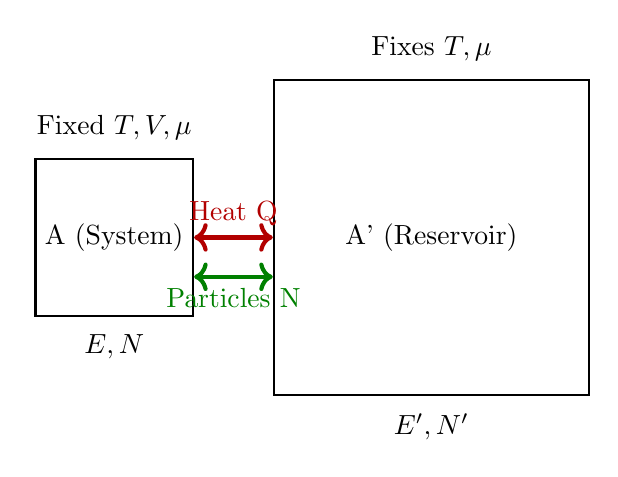
\begin{tikzpicture}
    \node (A) [draw, thick, minimum width=2cm, minimum height=2cm, label=center:A (System)] {};
    \node (Aprime) [draw, thick, minimum width=4cm, minimum height=4cm, right=1cm of A, label=center:A' (Reservoir)] {};
    % Interface allowing heat exchange & particle exchange
    \draw [line width=1.5pt, red!70!black, <->] (A.east) -- (Aprime.west) node [midway, above] {Heat Q};
    \draw [line width=1.5pt, green!50!black, <->] ($(A.east)+(0,-0.5)$) -- ($(Aprime.west)+(0,-0.5)$) node [midway, below] {Particles N};
    % Labels
    \node at (A.north) [above=0.1cm] {Fixed $T, V, \mu$};
    \node at (Aprime.north) [above=0.1cm] {Fixes $T, \mu$};
    \node at (A.south) [below=0.1cm] {$E, N$};
    \node at (Aprime.south) [below=0.1cm] {$E', N'$};
\end{tikzpicture}
\end{center}

The total system A+A' is closed and isolated:
$E + E' = E^{(0)} = \text{constant}$.
$N + N' = N^{(0)} = \text{constant}$.
Volumes $V, V'$ are fixed.

Equilibrium corresponds to maximum total entropy $S_{tot}(E, N) = S(E, N) + S'(E', N')$.
Consider variations $dE$ and $dN$ in system A. Then $dE'=-dE$ and $dN'=-dN$.
\[ dS_{tot} = dS + dS' \]
\[ dS_{tot} = \left[ \left(\pderiv{S}{E}\right)_N dE + \left(\pderiv{S}{N}\right)_E dN \right] + \left[ \left(\pderiv{S'}{E'}\right)_{N'} dE' + \left(\pderiv{S'}{N'}\right)_{E'} dN' \right] \]
\[ dS_{tot} = \left[ \left(\pderiv{S}{E}\right)_N - \left(\pderiv{S'}{E'}\right)_{N'} \right] dE + \left[ \left(\pderiv{S}{N}\right)_E - \left(\pderiv{S'}{N'}\right)_{E'} \right] dN \]
For $dS_{tot}=0$ in equilibrium for arbitrary $dE, dN$:
\begin{enumerate}
    \item $\left(\pderiv{S}{E}\right)_N = \left(\pderiv{S'}{E'}\right)_{N'} \implies \frac{1}{T} = \frac{1}{T'} \implies T=T'$. (Thermal equilibrium, as before).
    \item $\left(\pderiv{S}{N}\right)_E = \left(\pderiv{S'}{N'}\right)_{E'}$. (New condition for particle exchange equilibrium).
\end{enumerate}
We define the \textbf{Chemical Potential} $\mu$ such that:
\[ \frac{\mu}{T} \equiv - \left( \pderiv{S}{N} \right)_E \]
(Note the minus sign. $T$ in energy units, $S$ dimensionless, so $\mu$ has units of energy).
The new equilibrium condition becomes:
\[ -\frac{\mu}{T} = -\frac{\mu'}{T'} \]
Since $T=T'$, this implies:
\[ \mu = \mu' \]
Equilibrium between systems that can exchange energy and particles requires equality of temperature $T$ and chemical potential $\mu$.

\end{document}